\documentclass{article}

\usepackage[a4paper, total={6in, 8in}]{geometry}

\usepackage{amsmath}
\usepackage{amsfonts}
\usepackage{amssymb}
\usepackage[T1, T2A]{fontenc}
\usepackage[utf8]{inputenc}
\usepackage[english, russian]{babel}
\usepackage{graphics}
\usepackage{graphicx}

\geometry{
 a4paper,
 total={170mm,257mm},
 left=20mm,
 top=20mm,
 }

\author{Александр Валентинов}
\title{Лабораторная работа 3.6.1}

\begin{document}
   \subsection*{Работа 3.3.3}
   \section*{Опыт Милликена}
   
   \paragraph{Цель работы:} измерение элементарного заряда методом масляных капель

   \paragraph{В работе используются:} плоский конденсатор в защитном кожухе, осветитель, измерительный микроскоп, электростатический вольтметр, электронный секундомер, переключатель напряжения, пульверизатор с маслом.
   
   \subsubsection*{Экспериментальная установка:}
   
   \begin{figure}[h]
   \centering
   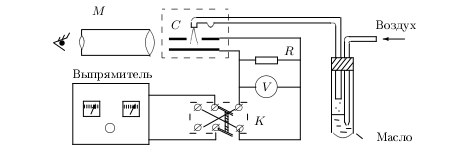
\includegraphics[width=10cm]{fig1.jpg} 
   \caption{Схема установки} 
   \label{fig.1} 
   \end{figure}

   \subsection*{Обработка результатов}
   Используя формулу
   \[ q = 9\pi\sqrt{\frac{2\eta^3 h^3}{g\rho}} \cdot \frac{l(t_0 + t)}{Vt_0^{3/2}t}, \]
   рассчитаем заряд каждой капли по средним значениям времен. При рассчете заряда будем складывать максимальную косвенную и случайную погрешности заряда. Отложим заряды капель по числовой оси.
   \begin{table} 
 \caption{Зависимость для RC-цепи}
 \label{RCtable}
\begin{center}
\begin{tabular}{|*{4}{r|}}
\hline 
$\psi$ & $\tan \psi$ & $\sigma_{\tan_\psi}$ & $1 / (\Omega C R_\Sigma)$ \\ \hline 
 1.51 & 16   & 1    & 25.7  \\ \hline 
 1.26 & 3.1  & 0.2  & 2.83  \\ \hline 
 1.01 & 1.6  & 0.1  & 1.65  \\ \hline 
 0.75 & 0.94 & 0.09 & 0.93  \\ \hline 
 0.50 & 0.55 & 0.07 & 0.566 \\ \hline 
 0.25 & 0.26 & 0.07 & 0.260 \\ \hline 
 0.00 & 0.00 & 0.06 & 0.099 \\ \hline 
 \end{tabular}
\end{center} 
\end{table} 

   \begin{figure}[h]
   \centering
   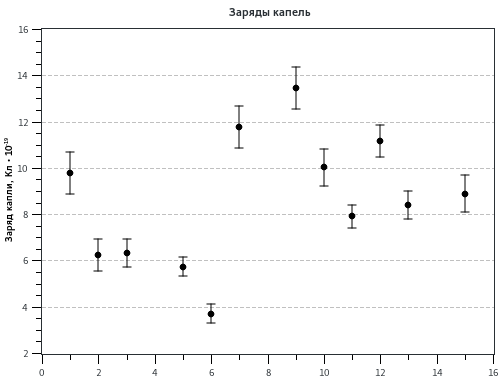
\includegraphics[width=10cm]{plot1.png} 
   \caption{Заряды капель} 
   \label{plot.1} 
   \end{figure}

   Сгруппируем капли так, чтобы через отрезки капель из одной группы можно было провести горизонтальную прямую.
   \begin{table} 
 \caption{Table2}
\begin{tabular}{|*{8}{c|}}
\hline 
I & Ex0.3 & Ex0.45 & Ex0.5 & Ex0.65 & Ex0.8 & Ex0.95 & Ex-0.95\\ \hline 
17.2 & 0 & 0 & 0 & 0 & 0 & 0 & 0 \\ \hline 
 181.9 & 0.051 & 0.072 & 0.084 & 0.109 & 0.129 & 0.159 & 0.166 \\ \hline 
 378.1 & 0.103 & 0.151 & 0.169 & 0.218 & 0.266 & 0.319 & 0.328 \\ \hline 
 571.8 & 0.151 & 0.224 & 0.251 & 0.322 & 0.396 & 0.472 & 0.496 \\ \hline 
 730.7 & 0.195 & 0.288 & 0.323 & 0.417 & 0.508 & 0.605 & 0.64 \\ \hline 
 854.4 & 0.228 & 0.336 & 0.378 & 0.487 & 0.595 & 0.71 & 0.75 \\ \hline 
 934.9 & 0.251 & 0.368 & 0.418 & 0.535 & 0.655 & 0.781 & 0.831 \\ \hline 
 1,003 & 0.269 & 0.394 & 0.446 & 0.569 & 0.698 & 0.83 & 0.884 \\ \hline 
 \end{tabular} 
\end{table} 
 
   
   Соотнесем группам целые числа так, чтобы мы получили линейную зависимость, построим график зарядов от этих чисел и найдем коэфициент наклона по методу наименьших квадратов.
   \begin{figure}[h]
   \centering
   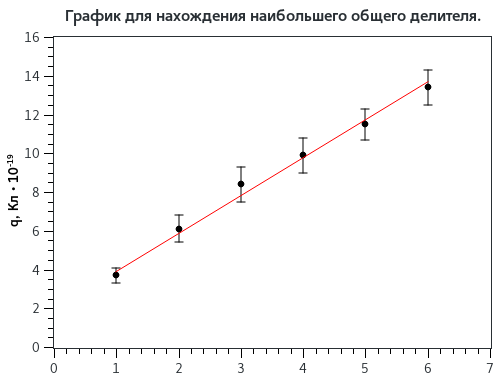
\includegraphics[width=10cm]{plot2.png} 
   \caption{График для нахождения НОД} 
   \label{plot.2} 
   \end{figure}

   Коэффициент наклона графика 
   \[ e = 1.95 \pm 0.15 \text{ Кл $\cdot 10^{-19}$} \]
   является наименьшим общим делителем зарядов.

   Заметим, что график пересекает ось $q$ в точке $q_0 \sim e$, значит в нашем эксперименте были капли заряда $2e$, но не было капель заряда $e$.

   Переведем величину $e$ в СГС:
   \[ e = 5.8 \pm 0.4 \text{ СГСЭ $ \cdot 10^{-10}$}. \]
   Заряд сходится с табличным значением по порядку величины.

   Оценим время релаксации:
   \[ \tau = \frac{v_{\text{уст}}}{g} = \frac{1}{g}\frac{h}{t_0} = 2.5 \text{мкс}. \]
   Путь, который пройдет капля за это время с установившейся скоростью:
   \[ s = v_{\text{уст}} \tau = 60 \cdot 10^{-10} \text{м}. \]
   \paragraph{Вывод} В ходе данной работы был измерен элементарный заряд, получившийся равным $1.95 \cdot 10^{-19}$ Кл, что сходится с табличными значениями. 
\end{document}
